\documentclass[a4paper]{article}
\usepackage[utf8]{inputenc}
\usepackage{graphicx}
\usepackage{onecolceurws}
\usepackage{xcolor}
\usepackage{url}
\usepackage{lineno}
\linenumbers


\def\infinity{\rotatebox{90}{8}}

\title{Un dataset internacional acerca de nombres, género y frecuencias en DameGender}

\author{
David Arroyo Menéndez, Madrid, Spain \\ \{davidam\@gmail\}.com
}

\newif\ifdraft
\drafttrue
%\draftfalse
\newcommand{\nb}[2]{
	{
		{\color{black}{
				\small\fbox{\bfseries\sffamily\scriptsize#1}
				{\sffamily\small$\triangleright~${\it\sffamily\small #2}$~\triangleleft$}
	}}}
}


\ifdraft
\newcommand\davidam[1]{\nb{David}{\color{olive}#1}}
\newcommand\grex[1]{\nb{Gregorio}{\color{red}#1}}
\newcommand\jgb[1]{\nb{Jesús{\color{blue}#1}}}
\newcommand\fixme[1]{{\textcolor{red}{[FIXME] #1}}}
\newcommand\cn{{\color{violet}[citation required]}}

\else
\usepackage[disable]{todonotes}
\newcommand\gema[1]{}
\newcommand\grex[1]{}
\newcommand\mei[1]{}
\newcommand\fixme[1]{}
\newcommand\cn{}


\fi
\let\labelindent\relax
\usepackage[inline]{enumitem}




\institution{DAMEGENDER}

\begin{document}

\maketitle

\begin{abstract}
  %% Introduction

  La igualdad de género es el quinto objetivo de desarrollo sostenible
  (ODS) para Naciones Unidas\footnote{https://www.un.org/sustainabledevelopment/gender-equality/}.

  Esta igualdad puede ser lograda midiendo, analizando datos y,
  creando buenas políticas con los resultados. Muchos estudios
  de género cuentan hombres y mujeres para explicar la posible
  desigualdad, por ejemplo, artículos de investigación, puestos
  de trabajo, calles, etc. El método tradicional de investigación
  es usar APIs comerciales con datos propietarios sin idea acerca
  de cómo los datos fueron recogidos. Los datos pueden también
  ser recogidos desde Wikipedia, estudios lingüísticos, sitios
  científicos, u oficinas estadísticas.

  %% Methodology

  Este enfoque está basado en recoger Datasets Abiertos (Open
  Datasets) que incluyen nombre, género y frecuencia desde
  muchas instituciones estadísticas. Así, las tareas abordadas
  están basadas en unificar formatos, procesar datos y, crear
  pruebas para medir la precisión de los nuevos datasets. 

  %% Results

  El dataset usado cubre más de 20 países en el mundo occidental
  trayendo miles de nombres con una precisión de acierto mayor del
  90\%. Esto permitirá medir brecha de género a estudiantes y
  académicos interesados en el fenómeno sin costes y de una manera
  reproducible y más personas estarán contribuyendo a eliminar la
  brecha de género.

  %% Conclusion

  El Software Libre y los datos provistos por instituciones estadísticas
  hacen posible producir investigación reproducible por pares.
  
\end{abstract}

\section{Introducción}
Naciones Unidas tiene como objetivo reducir la brecha de
género\footnote{https://www.un.org/sustainabledevelopment/gender-equality/},
para eso el primer paso es poder medir brecha de género
(``if you cannot measure it, you cannot improve it"~\cite{thompson1833electrical})
para medir brecha de género resulta económico utilizar ordenadores
(``Software Engineering Economics is an invaluable guide to determining
software costs, applying the fundamental concepts of microeconomics
to software engineering~\cite{barry1981software}'').

Además el software y los datos libres reducen más los costes, muchas personas
e instituciones utilizan Software Libre como LibreOffice o Ubuntu
GNU/Linux para evitar costes de licencias en productos similares
como Microsoft Windows o Microsoft Word.

Esto creará una competición en el mercado con algún ganador, evitando
pagos y generando beneficios desde una marca, tal y como ocurre en los
navegadores con Firefox y/o Chrome.

A través del uso de los nombres personales, uno puede inferir el sexo
o género de una persona en artículos académicos, libres, periódicos y muchas
interacciones en Internet. Así, detectar género desde los nombres puede
ser un camino estratégico para medir brecha de género, también.

Muchos usuarios y usuarias están, hoy en día, usando APIs tal y como
Genderize, GenderAPI, Namsor, NameApi, Wikipedia, u otras soluciones libres
(NLTK\cite{loper2002nltk}, R Gender, Gender Detector and Gender
Computer\footnote{https://github.com/tue-mdse/genderComputer}).

Las soluciones libres tradicionales tienen un bajo número de nombres debido
al uso de un solo fichero que quizás solo pertenece a un país siendo
software no mantenido a través del tiempo. Por otro lado, Wikipedia
almacena pocos nombres por país.

Sin embargo, la brecha de género es un problema reconocido en Naciones
Unidas y el mercado IT está liderando grandes desigualdades en economía
y brecha de género. Este artículo presenta datos recogidos para asistir
en la solución a un número de problemas (buscadores, inferiendo género en
ficheros CSV, nombres en diferentes países, creación de nuevos datasets)
encarados por la industria así como otros problemas que carecen de muchas
soluciones industriales como contar hombres y mujeres en GitHub, listas
de correo, etc.

Un estudio previo~\cite{karimi2016inferring} mostraba una comparativa de
datasets como un modo de mejorarla precisión, comparando herramientas que
usan diferentes datasets públicos
(SSA~\footnote{https://www.ssa.gov/oact/babynames/limits.html},
IPUMS~\footnote{https://usa.ipums.org/usa-action/variables/NAMEFRST},
namdict~\footnote{https://raw.githubusercontent.com/lead-ratings/gender-guesser/master/gender\_guesser/data/nam\_dict.txt},
etc).

Posibles aportaciones a este trabajo realizadas en este artículo
serían aumentar el número de nombres y la atención a la diversidad en
cuestiones como el género no binario o minorías culturales.

El dataset o quizás más bien DameGender (el software para crear el dataset)
podría ser aplicado en artículos de las diversas disciplinas donde operan
las herramientas de detección de género a partir del nombre~\cite{sun2019mitigating}:
ingeniería de software~\cite{vasilescu2012gender}, lingüística~\cite{hutson2016gender,al2009socio},
ciencias sociales~\cite{holman2018gender,mislove2011understanding,niemi2017gendered,de2014genero}),
... Con vocación de ser puntuados muchos de ellos como de ciencia
reproducible\cite{peng2011reproducible} si se tienen las precacuciones
correctas de la definición.

La estructura de este artículo es la siguiente:
La sección ~\ref{sec:stateofart} presenta la investigación principal midiendo brecha de género
y herramientas de detección de género desde el nombre.
La sección ~\ref{sec:design} da el vocabulario y la filosofía acerca de cómo elegir
fuentes y encarar las problemáticas de diversidad construyendo un
dataset
La sección ~\ref{sec:measuring} explica una aplicación para este dataset: medir brecha de
género en GNU/Linux
La sección ~\ref{sec:conclusions} es un resumen acerca de este enfoque y apunta a posibles
trabajos futuros.

Las contribuciones de este artículo son

1. Una solución integrada en los diferentes campos de aplicación relativos
a inferir género desde el nombre.

2. Una colección de datasets abiertos obtenidos desde fuentes estadísticas
estandarizadas en un formato único.

3. Un nuevo estudio para contar hombres y mujeres en GNU/Linux.

4. Un enfoque basado en resultados reproducibles.

Muchos artículos relacionados muestran técnicas de aprendizaje automático
aplicado, pero usando nuestro dataset libre mejoraría seguramente la
precisión de los resultados contrastada con diversas fuentes abiertas como Wikipedia,
Proyecto Gutenberg, Amazon, Forbes, instituciones deportivas, ... 

También recogidas en DameGender y, mejorando el Estado del Arte en lo que
respecta a Open Data en herramientas de detección de género a partir del
nombre de manera significativa al cubrir más de 20 países (figura \ref{fig:mapamundi})

\begin{figure}
  \centering
  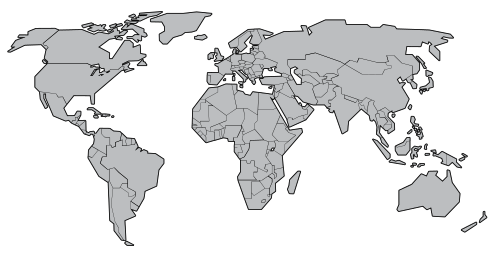
\includegraphics[width=0.6\textwidth]{images/Simple_world_map_edit.pdf}
  \caption[Caption for LOF]{Green (Countries with Open Data provided by Statistical Institutions), White (Countries without Open Data or don't reproduced by the author). Thanks to wikimedia by the mapamundi base source \url{https://commons.wikimedia.org/wiki/File:Simple_world_map_edit.svg}}
  \label{fig:mapamundi}
\end{figure}

\section{Estado del Arte}
\label{sec:stateofart}

\subsection{Acerca de la Brecha de Género}

Reducir la brecha de género se refiere a igualdad entre hombres y mujeres
y políticas de no discriminación. El género se refiere al sexo de la
persona determinado en su nacimiento, aunque éste pueda cambiarse en
algún momento de su vida. Las discusiones acerca de las definiciones
de género se refieren a estos problemas. Sin embargo, hay un consenso
determinando de género, frecuencia y nombres con estadísticas oficiales
entregadas por las instituciones de los estados.

Medir brecha de género requiere un conjunto de indicadores. Global Gender
Gap Report~\cite{chancel2022world} han sido propuesto en economía, salud,
educación y política. El sitio de Naciones Unidas\footnote{https://www.unwomen.org/}
está mostrando indicadores para medir disparidades como leyes, educación,
mortalidad maternal, participación política, pobreza, trabajo doméstico,
paridad de género en el trabajo, acceso a la economía, acceso a estudios
y/o trabajo, violencia contra las mujeres, justicia climática, acceso a
justicia, salud, etc.

Es posible crear decisiones de impacto en una cuestión a través de resultados
de investigación que toman estos indicadores en consideración. Por ejemplo,
Miyake y otros autores ~\cite{miyake2010reducing} concluyeron que creando
afirmaciones acerca de valores éticos la brecha de género se reducía en
los colegios.

Relativo a medir brecha de género en investigación social,
Bimber~\cite{bimber2000measuring} presentaba dos factores que afectan
a la brecha de género en Internet (acceso y uso), razones de socioeconomía
y género en una encuesta que recoge datos a través de varios años.

\subsection{Contando hombres y mujeres en Internet. ¿Por qué? ¿Dónde?}

El software DameGender focaliza en recuperar datos desde fuentes de datos
diversas acerca de género y nombres. Lugares como GitHub, Wikipedia, APIs,
periódicos, websites en general, listas de correo, ... Veamos cómo se
estaban haciendo estos trabajos.

Por ejemplo, un científico social estudiando brecha de género en
periodismo puede contar hombres y mujeres en Twitter. Mientras tanto,
algún artículo de ciencias de la computación puede estar mejorando la
detección de género en imágenes de caras, en nicknames, o simplemente
en nombres.

Burger y otros~\cite{burger2011discriminating} presentaron varias
configuraciones de un clasificador independiente de lenguaje para
predecir el género de usuarios Twitter. El dataset usado para la
construcción y evaluación de estos clasificadores se crea con usuarios
Twitter que llegaban a tener blog en su perfil.

Este tipo de estudios permite analizar demografía de población
Twitter~\cite{mislove2011understanding}, siendo del sexo una variable
clave en cualquier estudio de demografía. En este caso, el dataset
escogido fue el del censo de Estados Unidos que funciona razonablemente
bien para nombres occidentales.

Wagner y otros~\cite{wagner2015s} analizaban la brecha de género en
Wikipedia mostrando evidencia de pequeñas formas de desigualdad
explicando cómo resolver estas evidencias. Para medir la desigualdad
de género se han desarrollado las siguientes bias: visibilidad,
léxico (ej: palabras discriminatorias para mujeres), estructural y
de cobertura.

Un buen número de personas billonarias puntúan en Forbes como de
Ciencias de la Computación y los repositorios públicos nos permiten
entender tendencias de inclusión o no de mujeres, así como listados
públicos de puestos de trabajo, directivos, ... Las herramientas de
detección de género a partir del nombre. Arjona y
otros~\cite{10.1007/978-3-319-39225-7_13} publicaron en 2016 una
encuesta de 2000 contribuidores en el que la participación feminina
iría del 2\% al 5\%. Recientemente, Zacchiroli un estudio
longitudinal acerca de hombres y mujeres, que revelaba que las
mujeres podrían ser el 8\% en contribuciones de commits de código
en repositorios públicos. Zacchiroli~\cite{zacchiroli2020gender}
utilizó genderguesser para inferir género desde el nombre que a su
vez usa namdict~\footnote{https://raw.githubusercontent.com/lead-ratings/gender-guesser/master/gender\_guesser/data/nam\_dict.txt}
como dataset. Vasilescu y otros~\cite{vasilescu2015gender}
exploraron StackOverflow un sitio muy popular de preguntas y
respuestas concluyendo que los hombres representan la vasta
mayoría de contribuciones.

Relativo a la brecha de género en ciencia Cassidy R. Sugimoto
y otros~\cite{lariviere2013bibliometrics} presenta un análisis
bibliométrico confirmando que los desequilibrios de género
persisten en investigación a través del mundo entero. Holman
y otros~\cite{holman2018gender} presentaban un código en R
usando la API de genderize y proporciona un buen enfoque
acerca de cómo calcular brecha de género.

\subsection{Enfoques Automáticos para Inferir Género}

Hay varios caminos para inferir género desde fuentes de Internet:
texto escrito a mano, imágenes, documentos y nombres.

Liwicki y otros~\cite{liwicki2011automatic} presentaba un
método de inferir género desde textos escritos a mano con
un 67.5\%.

Gallagher y otros~\cite{gallagher2008estimating} presentaba
un trabajo que detecta género a partir de una combinación de
imágenes, edad e información cultural provista por primeros
nombres con ejemplos no etiquetados y con una precisión del
60\%.

Argamon y otros~\cite{argamon2003gender} explica que las
mujeres usan muchos más pronombres que los hombres, mientras
que los hombres usan más modificadores de nombres (determinantes,
o adjetivos). Koppel y otros~\cite{koppel2002automatically}
presentaban un sistema de clasificación de documentos con una
precisión del 80 \% aproximadamente. Cheng y otros~\cite{cheng2011author}
muestran una selección de características (features) y un
modelo construido usando aprendizaje automático generando
un acierto del 85.1 \% para identificar género desde el texto.

\subsection{Infiriendo género desde nombres}

Las herramientas usadas para inferir género desde un nombre
están normalmente basados en datasets que, como mínimo, incluyen
género.

Liu y otros~\cite{liu2013s} presentaba un método para inferir
género desde los primeros nombres en Twitter, el dataset estaba
codificado a mano por acuerdo entre tres trabajadores de Amazon
con 50.000 usuarios Twitter seleccionados aleatoriamente con
solo 12681 etiquetas de género. El objetivo de este estudio
era determinar el valor incremental de usar el nombre de
usuario (username) como una característica (feature) en la
inferencia de género basado en tweets.

Mueller y otros~\cite{mueller2016gender} presentaban un trabajo
de cómo inferir género en Twitter. Ellos usaban el dataset
namdict y el censo de los Estados Unidos como datasets.
Las características eran ``número de consonantes'', ``número de
vocales'', ``número de sílabas'', ``número de vocales bouba'',
``número de consonantes kiki'', ``número de vocales kiki''. El
modelo de clasificación era creado usando SVM.

\subsection{Ideas Relacionadas}

Ambekar y otros~\cite{ambekar2009name} presentaban un sistema de
software libre para clasificar nombre y etnicidad usando aprendizaje
automático para extraer una lista de nombres desde Wikipedia.
Un trabajo más reciente guiado por Rodríguez Pérez y
otros~\cite{nadri2021relationship}, en el que fue presentado
NamPrism dando ideas frescas acercar de clasificar razas y,
siendo aplicado a repositorios de software masivos.

Bollegala y otros~\cite{bollegala2010automatic} presentaba otro
enfoque que usaba basado en patrones léxicos para extraer aliases
de un nombre dado, con un conjunto de nombres y sus aliases
como datos de entrenamiento. Los aliases candidatos entran en un
ranking con varias puntuaciones. Support Vector Machine (SVM)
fue usado para construir la función ranking.

\subsection{Estándares Relacionados}

ISO/IEC 5218 propone la siguiente norma acerca de la codificación
de género: ``0 como conocido'', ``1 como masculino'', ``2 como femenino''
y ``9 como no aplicable''.

El RFC 6350 (vCard) tiene estas categorías ``m como masculino'',
``f como femenino'', ``0 como otro'', ``n como no aplicable'' y
``u como indefinido (undefined)''. Basado en este estándar, con
respecto a publicación web se puede usar el microformato h\_card
en el contexto de escribir interfaces de formularios web considerando
lecturas de w3.

\subsection{Resumen}

El primer nombre de un asunto es el factor clave usado para
determinar género en el Estado del Arte de las herramientas de
inferencia de género. Sin embargo, en muchos contextos hay más
características: apellidos, texto, imágenes, nicknames, etc.

El primer nombre puede ser útil para inferir otras cuestiones
tal y como raza, etnicidad, o cultura, también.

El aprendizaje automático y la selección de características
previas está siendo usado en muchos trabajos, aunque hay una
discusión tal que es el mejor enfoque.

\section{Diseño}

\subsection{Verdad y Falsedad en Nombres, Género y Frecuencia}

Usar nombre, género y frecuencia es una idea comúnmente admitida
en vez de otras enfoques como nombre y género, o nombre y varios
grados de masculinidad y feminidad. Esto es así, porque hay bastante
industria e instituciones que utilizan esta manera de hacer las cosas.
Así, las frecuencias nos permiten calcular porcentajes de masculinidad
y feminidad en cada nombre.

Con respecto, a veracidad en las datos DameGender permite elegir
a sus usuarios confiar en empresas o instituciones para inferir el
género de cualquier nombre.

Y, se aportan datasets públicos construidos desde instituciones
estadísticas que lo permiten. Este trabajo de observación de
datasets de instituciones oficiales tiene el potencial de favorecer
la participación ciudadana ante cambios desde los gobiernos.

\subsection{Género, Lenguaje, Nación y Diversidad}

Hay reglas y excepciones en diferentes lenguajes para predecir si
un nombre es masculino o femenino. Por ejemplo, en español o inglés,
hay más nombres que finalizan con ``a'' clasificadas como femeninos
que, como masculinos. Sin embargo, Andrea es femenino en España y,
masculino en Italia. Así, es útil comprender el lenguaje y cultura
asociado con un nombre. El lenguaje nos acerca a naciones, pero con
diferencias, por ejemplo, en España hay varios idiomas: vasco,
catalán, castellano (español) y gallego. Español es la lengua oficial
más utilizada en España, pero también en otros países como Argentina,
Méjico, Ecuador, Bolivia, ...

En DameGender se han juntado los datasets oficiales (los entregados
por instituciones estadísticas) para generar datasets de lenguajes.
En lenguajes donde no había instituciones estadísticas hemos valorado
utilizar nombres descargados de Wikipedia descubriendo una baja
cantidad de nombres una no muy buena calidad.

\subsection{Obteniendo datos y datasets para DameGender}

DameGender unificó los diferentes formatos descargados desde oficinas
estadísticas oficiales para nombre, género y frecuencia en los siguientes
países: Argentina, Austria, Australia, Bélgica, Canadá, Suiza, Alemania,
Dinamarca, España, Finlandia, Francia, Gran Bretaña, Irlanda, Islandia,
Noruega, Nueva Zelanda, Méjico, Portugal, Rusia, Eslovenia, Suecia,
Estados Unidos de América y Uruguay.

Se han desarrollado diferentes scripts para la descarga de datasets:
\begin{itemize}[noitemsep]
\item donwloadcsv.py: para la descarga de ficheros CSV desde las APIs
\item donwloadjson.py: para la descarga de ficheros JSON desde las APIs
\item get-wikidata-names.py: para la descarga de nombres desde Wikipedia
\item get-wikidata-surnames.py: para la descarga de apellidos desde Wikipedia
\item orig2.py: para la descarga de datasets desde instituciones estadísticas oficiales
\end{itemize}

Una posible mejora a este diseño sería unificar todas estas funcionalidades
en un solo comando, por ejemplo, orig2.py

%% These data reveals that the situation has been improved with respect
%% the long time. In \cite{10.1007/978-3-319-39225-7_13} speaks about a
%% female participation of around 2 {\%} to 5 {\%}.

\section*{Acknowledgments}

We would like to thank: the statistical institutions by
release of the open datasets about names, gender and frequency.
Luz Galvis for the software contributions, Daniel Izquierdo and
Laura Arjona for starting this research field at URJC all those
working with Jesús González Barahona and Gregorio Robles. 

\bibliographystyle{alpha}
\bibliography{uc3m}

\end{document}
